\appendix
\section{Model hyperparameters}\label{app:hyper}

The precise hyperparameters used for the various attentive models are as in
Table \ref{tab:hyper}. All models were trained using asynchronous RmsProp
\cite{Tieleman:2012:RMSPROP} with a momentum of $0.9$ and a decay of $0.95$.

\begin{table}[h]
  \centering
  \begin{tabular}{@{}lrrrr@{}}
    \toprule
    Model & Hidden Size & Learning Rate & Batch Size & Dropout \\
    \midrule
    Uniform, CNN & 256 & 5\ee{-}5 & 32 & 0.2 \\
    Attentive, CNN & 256 & 5\ee{-}5 & 32 & 0.2 \\
    Impatient, CNN & 256 & 5\ee{-}5 & 32 & 0.3 \\
    \midrule
    Uniform, Daily Mail & 256 & 5\ee{-}5 & 32 & 0.2 \\
    Attentive, Daily Mail & 256 & 2.5\ee{-}5 & 32 & 0.1 \\
    Impatient, Daily Mail & 256 & 5\ee{-}5 & 32 & 0.1 \\
    \bottomrule
  \end{tabular}
  \caption{Model hyperparameters}
  \label{tab:hyper}
\end{table}

\section{Performance across document length}\label{app:length}

To understand how the model performance depends on the size of the context, we
plot performance versus document lengths in Figures \ref{fig:patldec} and
\ref{fig:patl}. The first figure (Fig. \ref{fig:patldec}) plots a sliding window
of performance across document length, showing that performance of the attentive
models degrades slightly as documents increase in length. The second figure
(Fig. \ref{fig:patl}) shows the cumulative performance with documents up to
length $N$, showing that while the length does impact the models' performance,
that effect becomes negligible after reaching a length of \texttildelow 500~tokens.

\begin{figure}[h]
{\centering
  \begin{minipage}[t]{0.49\textwidth}
  \centering
  \includegraphics[scale=0.27,trim=0 0.1cm 0 1.8cm,clip=true]{{figs/pr_at_lendec.cnn}.png}
  \captionof{figure}{Precision@Document Length for the attention models on the CNN
    validation data. The chart shows the precision for each decile in document lengths
  across the corpus as well as the precision for the 5\% longest articles.}
  \label{fig:patldec}
\end{minipage}
% \hspace{0.15in}
\hfill
\begin{minipage}[t]{0.49\textwidth}
\centering
  \includegraphics[scale=0.27,trim=0 0.1cm 0 1.8cm,clip=true]{{figs/pr_at_len.cnn}.png}
  \captionof{figure}{Aggregated precision for documents up to a certain lengths.
  The points mark the $i^{th}$ decile in document lengths across the corpus.}
\label{fig:patl}
\end{minipage}
}
\end{figure}

\section{Additional Heatmap Analysis}

We expand on the analysis of the attention mechanism presented in the paper by
including visualisations for additional queries from the CNN validation dataset
below. We consider examples from the Attentive Reader as well as the Impatient
Reader in this appendix.

\subsection{Attentive Reader}

\paragraph{Positive Instances}
Figure \ref{fig:heatmapsA} shows two positive examples from the CNN validation
set that require reasonable levels of lexical generalisation and co-reference in
order to be answered.
The first query in Figure \ref{fig:heatmapsB} contains strong lexical cues
through the quote, but requires identifying the entity quoted, which is
non-trivial in the context document. The final positive example (also in Figure
\ref{fig:heatmapsB}) demonstrates the fearlessness of our model.

\begin{figure}[h]
  \centering
  \includegraphics[scale=0.30,clip=true,trim=3cm 17cm 3cm 2cm]{figs/goodexamples/174.png}%
  \includegraphics[scale=0.30,clip=true,trim=2cm 17cm 2cm 2cm]{figs/goodexamples/113.png}
  \caption{
	   Attention heat maps from the Attentive Reader for two more
           correctly answered validation set queries. Both examples
           require significant lexical generalisation and co-reference
           resolution to find the correct answers \textit{ent201} and
           \textit{ent214}, respectively.
       }
  \label{fig:heatmapsA}
\end{figure}

\begin{figure}[t]
  \centering
  \includegraphics[scale=0.30,clip=true,trim=3cm 27cm 2.2cm 2cm]{figs/goodexamples/130b.png}%
  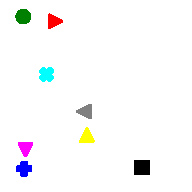
\includegraphics[scale=0.30,clip=true,trim=2cm 27cm 3cm 2cm]{figs/goodexamples/3.png}
  \caption{
    Two more
    correctly answered validation set queries. The left example (entity
    \textit{ent315}) requires correctly attributing the quote, which does not
    appear trivial with a number of other candidate entities in the vicinity.
    The right hand side shows our model is not afraid of Chuck Norris
    (\textit{ent164}).
  }
  \label{fig:heatmapsB}
\end{figure}

\paragraph{Negative Instances}
Figures \ref{fig:heatmapsC} and \ref{fig:heatmapsD} show examples of queries
where the Attentive Reader fails to select the correct answer. The two examples
in Figure \ref{fig:heatmapsC} highlight a fairly common phenomenon in the data,
namely ambiguous queries, where---at least following the anonymisation
process---multiple entities are plausible answers even when evaluated manually.
Note that in both cases the query searches for an entity marker that describes a
geographic location, preceded by the word ``in''. Here it is unclear whether
the placeholder refers to a part of town, town, region or country.

Figure \ref{fig:heatmapsD} contains two additional negative cases. The first
failure is caused by the co-reference entity selection process. The correct
entity, \textit{ent15}, and the predicted one, \textit{ent81}, both refer to the
same person, but not being clustered together. Arguably this is a difficult
clustering as one entity refers to ``Kate Middleton'' and the other to ``The
Duchess of Cambridge''.
The right example shows a situation in which the model fails as it
perhaps gets too little information from the short query and then selects the
wrong cue with the term ``claims'' near the wrongly identified entity
\textit{ent1} (correct: \textit{ent74}).

\begin{figure}[t]
  \centering
  \includegraphics[scale=0.3,clip=true,trim=3cm 32cm 2cm 2cm]{figs/badexamples/1.png}%
  \includegraphics[scale=0.3,clip=true,trim=2cm 32cm 3cm 2cm]{figs/badexamples/351b.png}
  \caption{
	   Attention heat maps from the Attentive Reader for two
           wrongly answered validation set queries. In the left case the model
           returns \textit{ent85} (correct: \textit{ent67}), in the right example
           it gives \textit{ent24} (correct: \textit{ent64}). In both cases the
           query is unanswerable due to its ambiguous nature and the model
           selects a plausible answer.
       }
  \label{fig:heatmapsC}
\end{figure}

\begin{figure}[t]
  \centering
  \includegraphics[scale=0.3,clip=true,trim=3cm 30cm 2cm 2cm]{figs/badexamples/10.png}%
  \includegraphics[scale=0.3,clip=true,trim=2cm 30cm 3cm 2cm]{figs/badexamples/15.png}
  \caption{
	   Additional heat maps for negative results. Here the left query
           selected \textit{ent81} instead of \textit{ent15} and the right query
           \textit{ent1} instead of \textit{ent74}.
         }
  \label{fig:heatmapsD}
\end{figure}


\subsection{Impatient Reader}

To give a better intuition for the behaviour of the Impatient Reader, we use a
similar visualisation technique as before. However, this time around we
highlight the attention at every time step as the model updates its focus while
moving through a given query. Figures \ref{fig:heatmapsE}--\ref{fig:heatmapsZ} shows how the attention
of the Impatient Reader changes and becomes increasingly more accurate as the
model considers larger parts of the query.
Note how the attention is distributed
fairly arbitraty at first, slowly focussing on the correct entity
\textit{ent5} only once the question has sufficiently been parsed.

\begin{figure}[h]
  \centering
  \setlength{\fboxsep}{0pt}

  \fbox{\includegraphics[scale=0.22,clip=true,trim=3cm 27cm 3cm 2.5cm]{figs/framesvideo/22f1.png}}%
  \fbox{\includegraphics[scale=0.22,clip=true,trim=3cm 27cm 3cm 2.5cm]{figs/framesvideo/22f2.png}}%
  \fbox{\includegraphics[scale=0.22,clip=true,trim=3cm 27cm 3cm 2.5cm]{figs/framesvideo/22f3.png}}
  \caption{Attention of the Impatient Reader at time steps 1, 2 and 3.}
  \label{fig:heatmapsE}
\end{figure}

\begin{figure}[h]
  \centering
  \setlength{\fboxsep}{0pt}

  \fbox{\includegraphics[scale=0.22,clip=true,trim=3cm 27cm 3cm 2.5cm]{figs/framesvideo/22f4.png}}%
  \fbox{\includegraphics[scale=0.22,clip=true,trim=3cm 27cm 3cm 2.5cm]{figs/framesvideo/22f5.png}}%
  \fbox{\includegraphics[scale=0.22,clip=true,trim=3cm 27cm 3cm 2.5cm]{figs/framesvideo/22f6.png}}
  \caption{Attention of the Impatient Reader at time steps 4, 5 and 6.}
\end{figure}

\begin{figure}[h]
  \centering
  \setlength{\fboxsep}{0pt}

  \fbox{\includegraphics[scale=0.22,clip=true,trim=3cm 27cm 3cm 2.5cm]{figs/framesvideo/22f7.png}}%
  \fbox{\includegraphics[scale=0.22,clip=true,trim=3cm 27cm 3cm 2.5cm]{figs/framesvideo/22f8.png}}%
  \fbox{\includegraphics[scale=0.22,clip=true,trim=3cm 27cm 3cm 2.5cm]{figs/framesvideo/22f9.png}}
  \caption{Attention of the Impatient Reader at time steps 7, 8 and 9.}
\end{figure}

\begin{figure}[h]
  \centering
  \setlength{\fboxsep}{0pt}

  \fbox{\includegraphics[scale=0.22,clip=true,trim=3cm 27cm 3cm 2.5cm]{figs/framesvideo/22f10.png}}%
  \fbox{\includegraphics[scale=0.22,clip=true,trim=3cm 27cm 3cm 2.5cm]{figs/framesvideo/22f11.png}}%
  \fbox{\includegraphics[scale=0.22,clip=true,trim=3cm 27cm 3cm 2.5cm]{figs/framesvideo/22f12.png}}
  \caption{Attention of the Impatient Reader at time steps 10, 11 and 12.}
  \label{fig:heatmapsZ}
\end{figure}
